\begin{problem}{아기새}
	{standard input}{standard output}
	{3 seconds}{24 megabytes}{}
	
	몇년간의 노력 끝에, 범수는 결국 조종사면허를 탔다. 이 사실을 기념하기 위해 그는 항공기를 사서 자신이 사는 행성인 \textbf{3-샛}별 근처를 비행하려고 한다. 구체적으로, 범수는 적도 근처를 한바퀴 비행하려고 한다. 불행하게도, 행성이 매우 크기 때문에 중간에 연료를 재충전하는것이 필요하다. 각 항공기가 연료가 꽉 찬 상태에서 얼마나 멀리 비행할 수 있는지가 알려져 있다. 적도 근처에는 많은 수의 공항이 있고 항공기가 공항에 착륙하면 연료를 충전할 수 있다. 항공기를 사는것은 중요한 일이길 때문에, 범수는 당신의 도움을 요청했다. 그는 자신이 구매를 생각하는 다양한 항공기 종류를 알려줄 것이다. 각 항공기들은 한번에 얼마나 멀리 비행할 수 있는지가 다르다. 각 항공기 모델에 따라 여행을 하기 위한 최소한의 (마지막 착륙을 포함한) 착륙 횟수가 궁금해 졌다. 각 항공기 모델에 따라, 여행은 자신이 원하는 각자 다른 공항에서 시작할 수도 있다.
	
	\InputFile
	
	입력의 첫째 줄에는 적도에 있는 공항의 수 $n$과 범수가 구매를 생각하는 항공기 종류의 수 $s$가 공백 하나로 구분되어 주어진다. ($2 \le n \le 1,000,000$, $1 \le s \le 100$).
	
	둘째 줄에는 공항 간의 간격을 의미하는 $n$개의 양의 정수 $l_1$, $l_2$, $\cdots$, $l_n$이 공백 하나로 구분되어 주어진다. ($l_1 + l_2 + \cdots + l_n \le 10^9$) $l_i$는 $i$번째 공항과 $i+1$번째 공항($i = n$인 경우는 $n$번째 공항과 첫번째 공항)의 거리를 km단위로 의미한다.
	
	셋째 줄에는 $s$개의 정수 $d_1$, $d_2$, $\cdots$, $d_s$ ($1 \le d_i \le l_1 + l_2 + \cdots + l_n$)가 공백 하나로 구분되어 주어진다. $d_i$는 착륙 하지 않고 비행기가 날 수 있는 거리를 km단위로 의미한다.
	
	
	
	\OutputFile
	
	프로그램은 $s$개의 줄을 출력해야 한다. $i$번째 줄에는 3-샛별을 적도를 따라 한바퀴 돌기 위한 최소한의 이착륙 횟수를 나타내는 정수 하나를 출력하거나, 비행이 불가능 하면 \texttt{NIE}를 출력해야 한다.
	
	\SubtaskWithCost{1}{20}
	\begin{itemize}
		\item $n \le 1,000$
	\end{itemize}
	
	\SubtaskWithCost{2}{30}
	\begin{itemize}
		\item $n \le 100,000$
	\end{itemize}
	
	\SubtaskWithCost{3}{18}
	\begin{itemize}
		\item $s \le 5$
	\end{itemize}
	
	\SubtaskWithCost{4}{32}
	추가 제한 조건이 없다.
	
	
	
	\Examples
	
	\begin{example}
	\exmp{
	6 4
	2 2 1 3 3 1
	3 2 4 11
	}{%
	4
	NIE
	3
	2
	}%
\end{example}

\Note
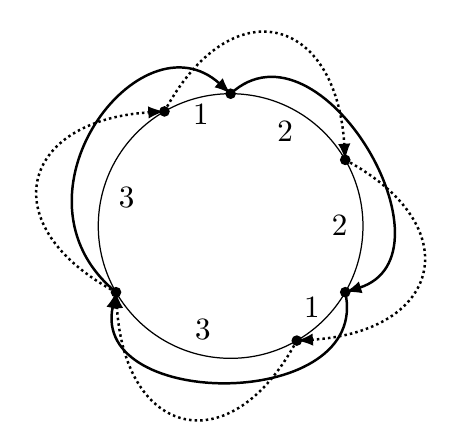
\includegraphics[]{doo.png}

실선은 착륙하지 않고 비행기가 날 수 있는 거리가 4km일 때의 최적의 비행을 보여준다. 점선은 3km 일 때 이다.
\end{problem}

